\documentclass[tikz]{standalone}

\usepackage{times}
\usepackage{pgfplots}
\pgfplotsset{compat=1.18}
\usepgfplotslibrary{fillbetween}
% \usepgfplotslibrary{patchplots}

\begin{document}

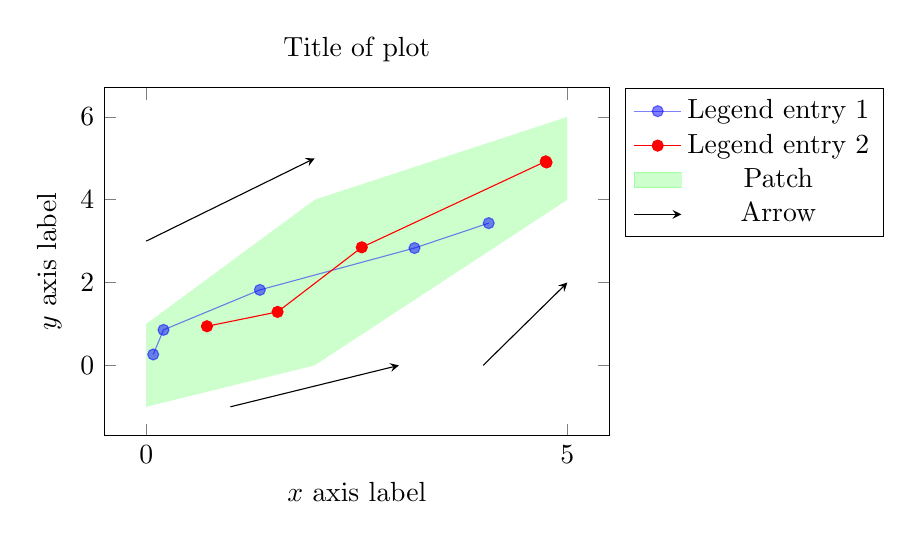
\begin{tikzpicture}
\begin{axis}[
    title={Title of plot},
    xlabel={$x$ axis label},
    ylabel={$y$ axis label},
    % xmin=0,
    % xmax=100,
    % ymin=0,
    % ymax=120,
    % xtick={0, 5},
    % ytick={0, 5},
    xtick distance=5,
    ytick distance=2,
    % xticklabels={,,},
    % yticklabels={,,},
    legend pos=outer north east,
    % legend pos=north west,
    % xmajorgrids=true,
    % ymajorgrids=true,
    % grid style=solid,
    width=8cm,
    height=6cm,
    % width=4cm,
    % height=3cm,
    shader=flat corner,
]

    \addplot[color=blue, mark=*, opacity=0.5]
        coordinates {(0.083,0.263)(0.205,0.857)(1.349,1.822)(3.185,2.833)(4.066,3.434)};
        \addlegendentry{Legend entry 1}

    \addplot[color=red, mark=*, opacity=1]
        coordinates {(0.721,0.944)(1.559,1.291)(2.559,2.850)(4.743,4.926)(4.752,4.899)};
        \addlegendentry{Legend entry 2}

    \addplot[name path=y1, opacity=0, forget plot]
        coordinates{(0,-1)(2,0)(5,4)};

    \addplot[name path=y2, opacity=0, forget plot]
        coordinates{(0,1)(2,4)(5,6)};

    \addplot[green, opacity=0.2]
        fill between[of=y1 and y2];
        \addlegendentry{Patch}

    \addplot[
        quiver={
            u=\thisrow{u},
            v=\thisrow{v},
        },
        -stealth,
    ]
        table {
            x  y  u  v
            1 -1  2  1
            4  0  1  2
            0  3  2  2
        };
        \addlegendentry{Arrow}

\end{axis}
\end{tikzpicture}

\end{document}
